
\documentclass[unknownkeysallowed]{beamer}
\usetheme{Madrid}
\usepackage{subfig}
\usepackage{xcolor}
\usepackage{wrapfig}
\usepackage{mathtools}
\usepackage{braket}
\usepackage{fourier}

\title{Dimensionality reduction with UMAP}
\subtitle{Advanced Data Mining seminar}
\author{Jakub Bartczuk}
\centering
\date{March 2020}
\begin{document}
\maketitle

\begin{frame}{Overview}
	\tableofcontents[section,subsection]
\end{frame}

\begin{frame}{Teaser}
	\framesubtitle{Reducing dimensionality of COIL20 Dataset}
	\begin{figure}[ht]\centering\begin{minipage}[b]{0.45\linewidth}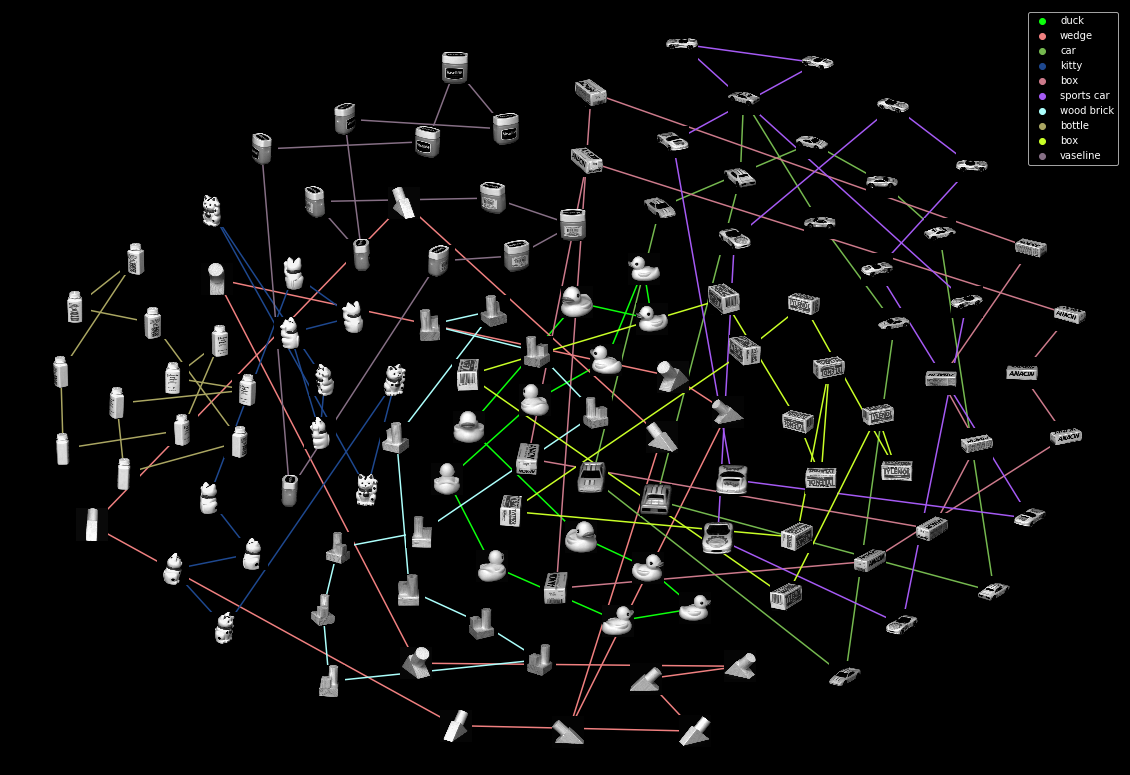
\includegraphics[width=\textwidth]{coil_tsne.png}\caption{tSNE}\label{fig:minipage1}\end{minipage}\quad\begin{minipage}[b]{0.45\linewidth}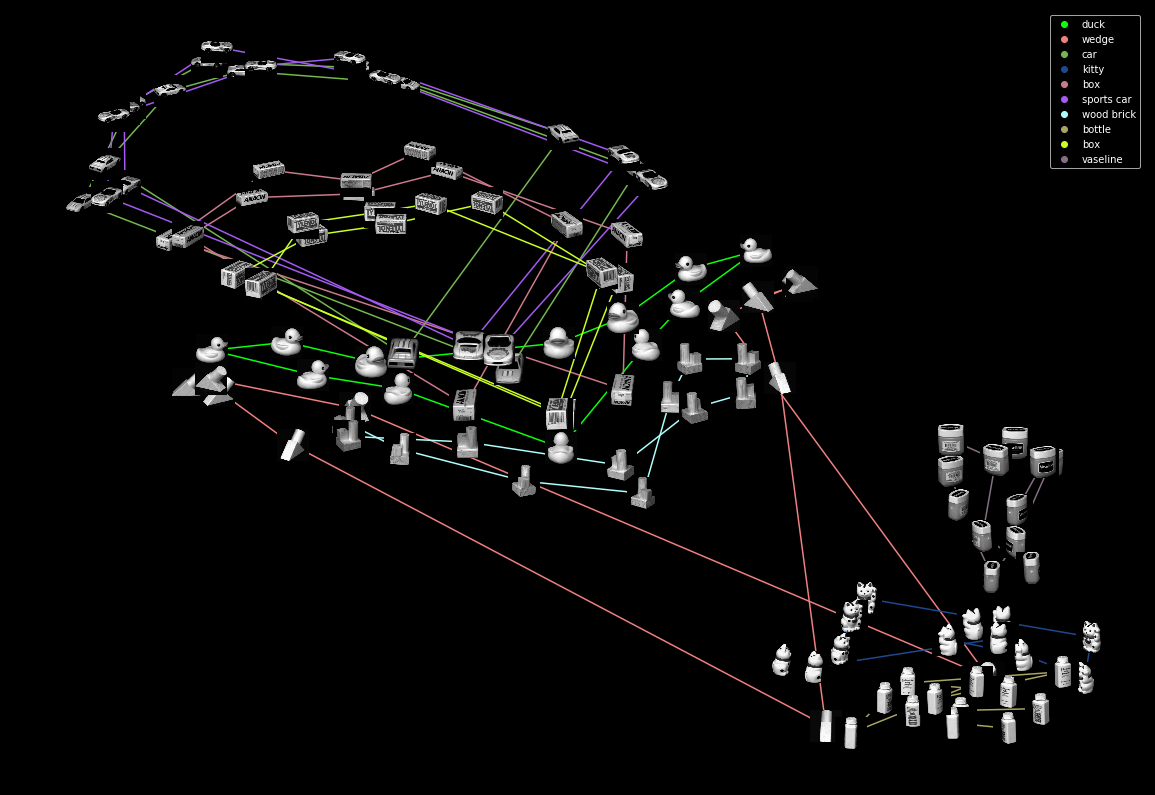
\includegraphics[width=\textwidth]{coil_umap.png}\caption{UMAP}\label{fig:minipage2}\end{minipage}\end{figure}
\end{frame}

\section{Manifold learning recap}
\begin{frame}{Manifold learning recap}

	\begin{itemize}
	\item We want to uncover lower-dimensional structure in high-dimensional space
	\item Is the structure linear? If yes, use PCA
	\item What to do if it is not linear?
	\end{itemize}
\end{frame}
\begin{frame}{Manifold learning recap}



	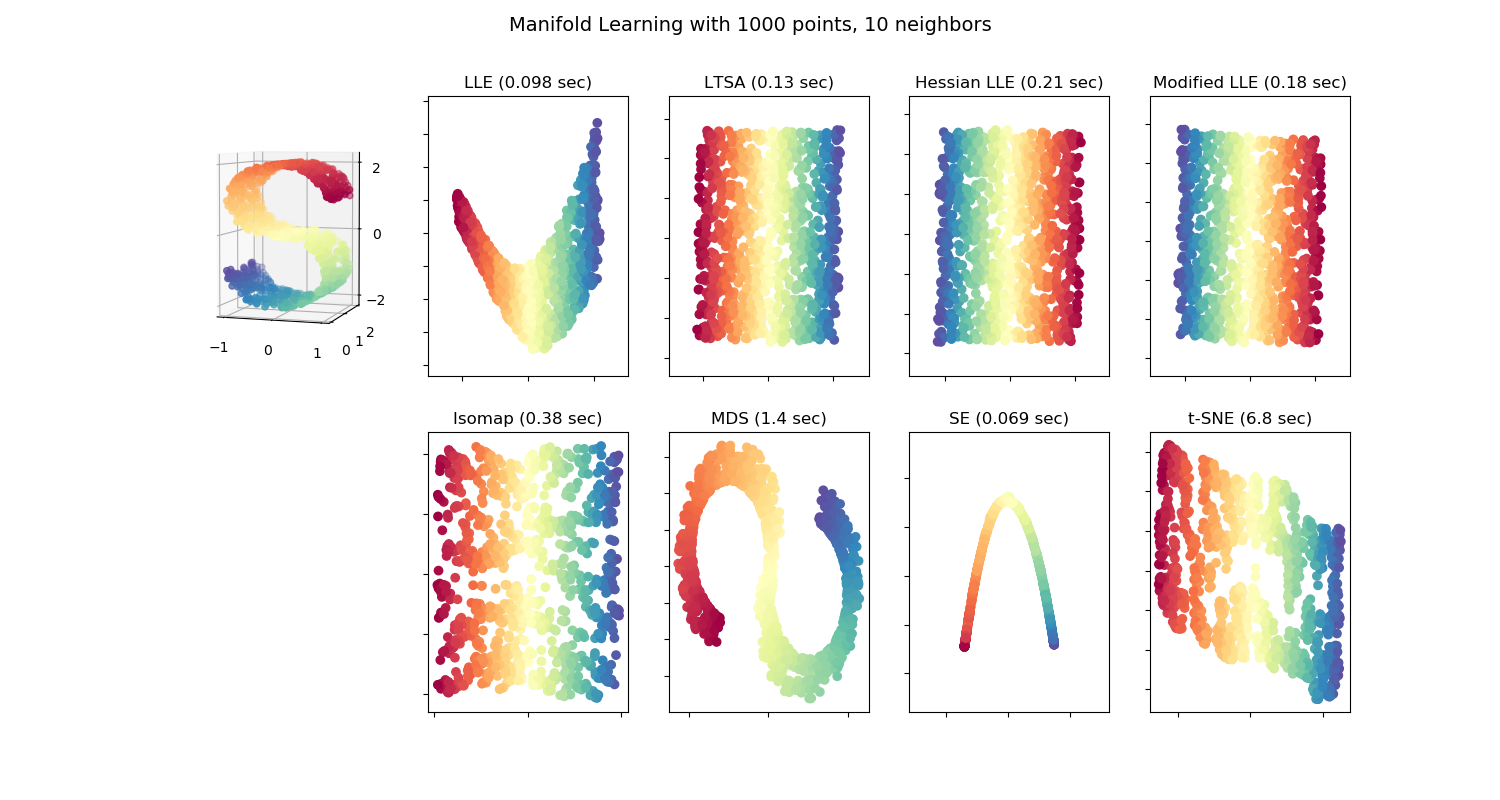
\includegraphics[width=\textwidth,height=0.8\textheight,keepaspectratio]{manifold_algorithms}

\end{frame}

\subsection{Multidimensional Scaling}
\begin{frame}{Classical Multidimensional Scaling}


	$$D_{i,j} = \|x_i - x_j\|^2$$

	Find $y$'s, $D'_{i,j} = \|y_i - y_j\|^2$ 

	Such that $D' \approx D$

\end{frame}


\begin{frame}{Classical MDS properties}

	\begin{itemize}[<+->]
		\item easy to compute - decompose low-rank matrix from D
		\item fast - Euclidean distance matrix just couple of vectorized matrix computations
		\item treats all distortions alike
	\end{itemize}



	\begin{block}<+->{What structure does MDS preserve?}
	The last property basically means that we preserve local and global structure alike.

	\begin{itemize}
		\item $x$'s are close - they are close in embedding.
		\item $x$'s are distant - they are equally distant in embedding.
	\end{itemize}

	\end{block}
\end{frame}
\subsection{Distances, graphs and matrix decomposition}

\begin{frame}{Distances, graphs and matrix decomposition}

	\begin{block}{Local vs global structure}
	We may not care about preserving exact large distances in embedding space as much as small distances

	\textcolor{red}{Idea}: Calculate distance along the set 'spanned' by datapoints
	\end{block}

	\begin{block}{Manifold hypothesis}
	The data lies in lower-dimensional, possibly nonlinear space which is embedded in ambient space
	\end{block}



\end{frame}

\begin{frame}{MDS breakdown}


	\begin{enumerate}
	   \item estimate distances between some pairs of close points
	   \item make graph $(X, E)$ with edges weighted by distance
	   \item define $D$ as distance from graph
	   \item decompose matrix that represents the graph
	\end{enumerate}{}

	\begin{block}<2->{Getting manifold learning algorithms from schematic}

	\begin{itemize}
		\item Setting $E = \{((x_i, x_j), \|x_i - x_j\|^2) | x_i, x_j \in X \}$ (complete graph) we get classical MDS
		\item Modifying steps 1-3 will get us Isomap, Hessian Eigenmaps
		\item tSNE and UMAP will change step 4
	\end{itemize}
	\end{block}



\end{frame}

\section{Stochastic Neighbor Embedding}
\begin{frame}{Stochastic Neighbor Embedding}

	Idea: embed into lower-dimensional space, preserve distance statistics

	$$q_{j|i} = \frac{\textcolor{blue}{f}(\|y_i - y_j\|)}{\sum_{k \neq j}\textcolor{blue}{f}(\|y_i - y_k\|)}, p_{j|i} = \frac{exp(-\|x_i - x_j\|^2 / \textcolor{red}{s^2_i})}{\sum_{k \neq j}exp(-\|x_i - x_k\|^2/\textcolor{red}{s^2_i})}$$

	$$KL(p, q) = \sum_{i, j} p_{j|i} log\frac{p_{j|i}}{q_{j|i}}$$

	\begin{block}{Notes}
	Choice of $\textcolor{blue}{f}$ determines algorithm:
	\begin{itemize}
		\item $\textcolor{blue}{f(x) = exp(-x^2)}$ - original SNE
		\item $\textcolor{blue}{f(x) = (1 + x^2)^{-1}}$ - tSNE (note this is density of Cauchy distribution up to a constant)
	\end{itemize}
	\end{block}
\end{frame}

\begin{frame}{Stochastic Neighbor Embedding}

	\begin{block}{Perplexity}
	\textcolor{red}{$s$} gives rise to perplexity $P_i = 2^{H(p_i)}$ which controls effective neighborhood size at $x_i$.
	\end{block}

	\begin{block}{High level algorithm}
	\begin{itemize}
		\item for each $x_i$ find $s$ that matches given perplexity
		\item initialize $y_i$ randomly
		\item minimize KL with gradient descent w.r.t. $y_i$
	\end{itemize}
	\end{block}

\end{frame}


\begin{frame}{Problems with SNE: Crowding problem}

	\begin{columns}[onlytextwidth]
	\begin{column}[T]{.48\textwidth}
	\begin{itemize}[<+->]
		\item 'more room' for intermediate distances in higher dimensions

		\item pairs of points will tend to have similar distance (\textcolor{red}{remember curse of dimensionality for kNN})
		\item harder to embed them faithfully into lower dimensional space

	\end{itemize}
	\end{column}

	\begin{column}[T]{.48\textwidth}
	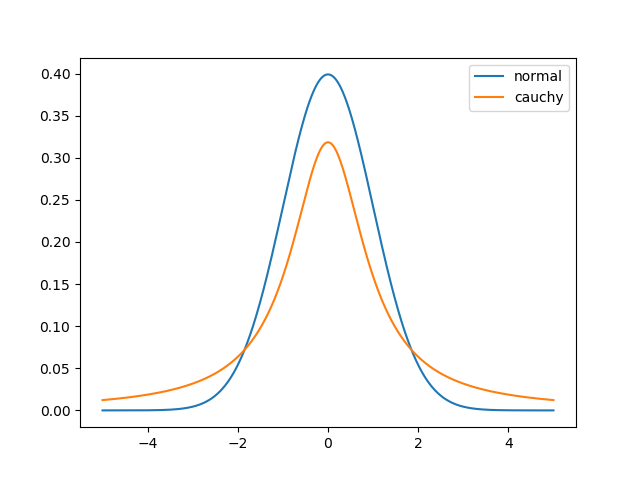
\includegraphics[width=\textwidth]{long_tail.png}
	\end{column}
	\end{columns}

	\begin{itemize}
	\item<4-> somewhat fixed by using t Distribution which has longer tails (not so concentrated around maximum).

	This problem is not specific to tSNE - it relates to the fact that data may not be sampled uniformly from manifold
	\end{itemize}

\end{frame}

\section{UMAP}


\begin{frame}{Bird's view of UMAP's theory}

	\begin{flushleft}
	Recall UMAP means \textbf{Uniform} Manifold Approximation and Projection
	\end{flushleft}

	
	\begin{block}{Algorithm}
		\begin{enumerate}
		\item get input data representation
		\item initialize embedding
		\item calculate probabilities of points being nearest neighbors
		\item optimize  embedding
		\end{enumerate}
	\end{block}
	\begin{block}<2->{This also describes tSNE, what are the differences?}
	\begin{enumerate}
		\item Fuzzy set built using local distance functions ( Riemannian metric)
		\item kNN graph's Laplacian
		\item Probability between points corresponds to likelihood of points being connected in neighborhood graph
		\item Cross entropy between fuzzy sets
	\end{enumerate}
	\end{block}

\end{frame}

\begin{frame}{UMAP vs tSNE in a nutshell}
\framesubtitle{UMAP paper appendix C}

	{\scalebox{1.3}{
	\begin{tabular}{c|c|c}
	 & UMAP & tSNE \\
	 \hline
	 {\tiny Initialization} &  {\tiny Laplacian decomposition} & {\tiny Random Gaussian} \\
	 \hline
	 {\tiny Optimization} & {\tiny SGD + negative sampling} & {\tiny Gradient Descent} \\
	 \hline
	 $p_{i|j}$ & $exp(- \frac{d(x_i, x_j) - \textcolor{green}{\rho_i}}{\textcolor{red}{\sigma_i}})$ & $\frac{exp(-\|x_i - x_j\|^2 / \textcolor{red}{s^2_i})}{\sum_{k \neq j}exp(-\|x_i - x_k\|^2/\textcolor{red}{s^2_i})}$ \\
	 \hline
	 $q_{i|j}$ & \textcolor{blue}{$(1 + a\|y_i - y_j\|^{2b}))^{-1}$} & $\frac{(1 + (\|y_i - y_j\|^2))^{-1}}{\sum_{k \neq j}(1 + (\|y_i - y_k\|^2))^{-1}}$ \\
	 \hline
	 {\tiny Loss} & {\tiny H(q, p) = H(p) + KL(q, p)} & {\tiny KL(q, p)}
	\end{tabular}
	}
	}
	\begin{block}{Why such p, q?}
	\begin{itemize}
		\item \textcolor{green}{$\rho_i$} - Riemannian structure
		\item \textcolor{red}{$\sigma_i$} - analogous to \textcolor{red}{$s_i$}
		\item \textcolor{blue}{$q$} - approximation of membership for fuzzy simplicial complex
	\end{itemize}
	\end{block}
\end{frame}



\subsection{Topological and geometrical preliminaries}

\begin{frame}{Riemannian structure}

	Remember we want to calculate distance \textbf{along the manifold} 

	\begin{block}<1->{Curve length in Euclidean space}

	$L_\gamma = \int_{0}^{1} \|\gamma'(t)\| dt =  \int_{0}^{1} \sqrt{\braket{\gamma'(t) | \gamma'(t)}} dt$

	\end{block}

	\begin{block}<2->{Definition}

	\textit{Riemannian space} has local inner product.

	Precisely, it has an inner product on each tangent space that varies smoothly.
	\end{block}

	\begin{block}<3->{Idea}
	Estimate Riemannian structure locally with finite samples - set it constant on neighborhoods
	\end{block}
	
	\begin{alertblock}<3->{Problem}
	We get incompatible local structures
	\end{alertblock}
\end{frame}

\begin{frame}{Riemannian structure}
	\includegraphics[width=\paperwidth]{local_metric.png}
\end{frame}

%% OPTIONAL

\begin{frame}{Some Category Theory}

	Category theory is not a theory per se, it's rather a framework for thinking about mathematics

	\begin{block}{Definitions}
	A \textit{category} $\mathcal{C}$ is a collection of objects with \textit{morphisms} that can be composed and the composition satisfies some technical conditions

	\end{block}

	Think a set of some sets with functions that preserve structure

	\begin{block}{Definition}
	A morphism $f: A \to B$ is an \textit{isomorphism} if there is a morphism $g: B \to A$ such that $f \circ g = id_A$ and $g \circ f = id_B$
	\end{block}

\end{frame}

\begin{frame}{Some Category Theory}

	\begin{exampleblock}{Examples}
	\begin{itemize}
		\item category $FinSet$ of finite sets and functions between them
		\item category $Graphs$ of graphs and graph homomorphisms
		\item category $Ab$ of Abelian groups and group homomorphisms
		\item category of metric spaces and contractions
	\end{itemize}
	\end{exampleblock}

	\begin{block}{Definition}
	A mapping $F: \mathcal{C} \to \mathcal{D}$ is a \textit{functor} if $F(f \circ g) = F(f) \circ F(g)$

	Warning: technically this is a pair of mappings but we usually omit this
	\end{block}

	\begin{exampleblock}{Examples}
	$F: Graphs \to FinSet$ $F((V,E)) = V$
	\end{exampleblock}

\end{frame}

\begin{frame}{Topological preliminaries}

    \begin{block}{Extended pseudometric space}
    A space is called \textit{pseudometric} if it suffices metric space axioms, but without requiring that $d(x, y) = 0 \implies x = y$


    $d: X \times X \to \mathbb{R}^+$
    \begin{itemize}
        \item $d(x,y) = d(y, x)$
        \item $d(x, y) + d(y, z) \geq d(x, z)$

    \end{itemize}

    In  \textit{extended pseudometric space} it also can happen that $d(x, y) = \infty$

    \end{block}

\end{frame}


\begin{frame}{Topological preliminaries}

	\begin{columns}[T]
	\begin{column}{0.5\linewidth}

	\begin{block}{Simplex}
	A $d$-dimensional simplex is a set $S \subset \mathbb{R}^n$ such that there are $d$ linearly independent points $S = conv(d)$ 

	\end{block}

	\begin{block}{Simplicial complex}
	A set $C$ of simplexes such that if $s, s' \in C \implies s \cap s' \in C$ 
	\end{block}
	\end{column}
	\begin{column}{0.5\linewidth}
	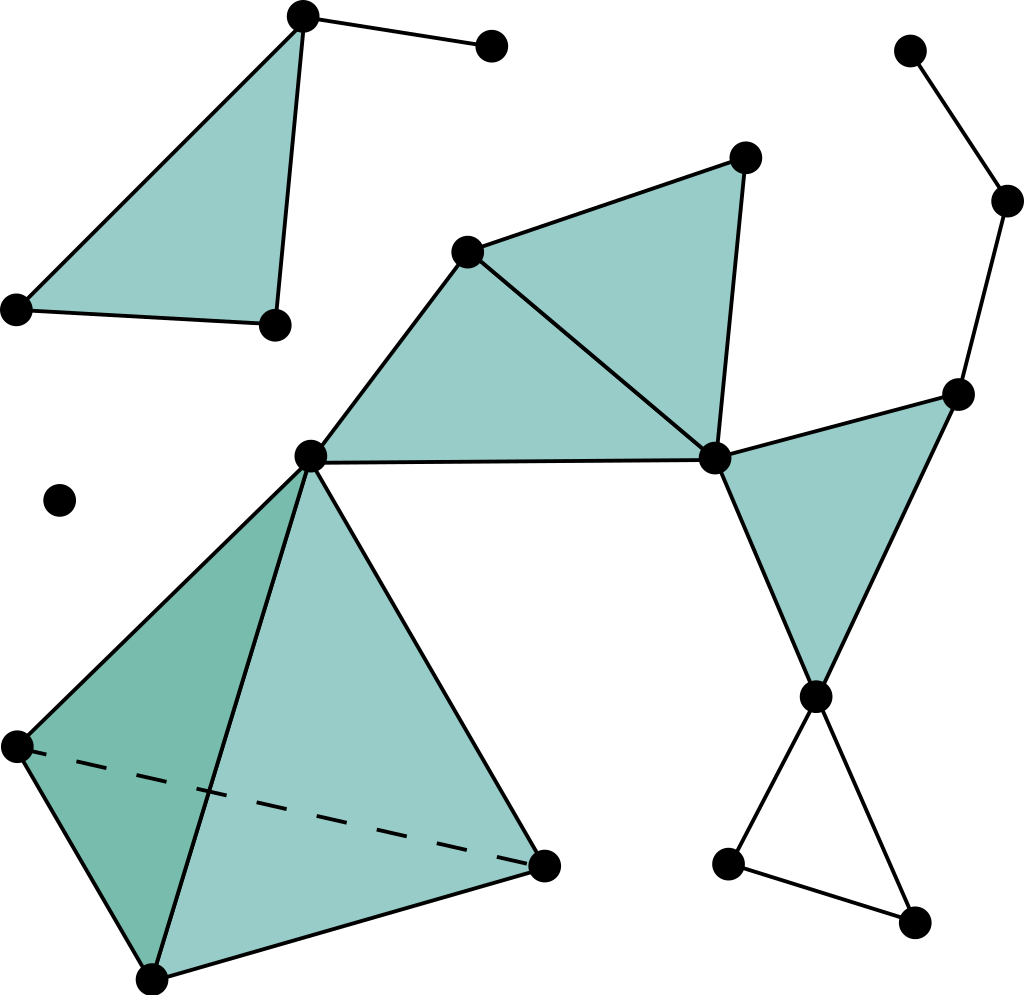
\includegraphics[width=\textwidth,height=0.5\textheight,right]{Simplicial_complex_example.svg.png}

	\end{column}
	\end{columns}
\end{frame}



\begin{frame}{Topology}

	\begin{block}{Definition}
	Definition: \textit{nerve} of a family of sets $\mathcal{U} = \{U_i| i \in I \}$ is the set of finite subsets $s$ of $I$ for which $\bigcap_{i \in s} U_i \neq \emptyset$
	\end{block}

	\begin{block}{Definition}

	$\mathcal{U}$ is a \textit{cover} of $X$ if $\bigcup_i U_i = X$
	\end{block}

	\begin{block}{Nerve theorem}

	If set $\mathcal{U}$ is an open cover of $X$  then $X \sim N(\mathcal{U})$ (they are homotopy equivalent, this is one notion of equivalence from topology)

	\end{block}
\end{frame}

\begin{frame}{Fuzzy sets}

    \begin{block}<1->{Definitions}
    For fixed set $X$, $S \subset X$, $m: S \to [0, 1]$ (fuzzy membership function)
    \break
    A pair $(S, m)$ is a \textit{fuzzy set} if $0 \leq m(x) \leq 1$

    Fuzzy sets have natural generalizations of set operations: 
    \break
    if $(S, m_S), (R, m_R)$ are fuzzy sets then 
    \break
    $(S \cup R, m_{S \cup R})$ is a fuzzy set
    \break
    where
    \break
    $m_{S \cup R}(x) = max(m_S(x), m_R(x))$
    \end{block}

    \begin{exampleblock}<2->{Example}

    $S_1 = ([0, 1], m)$, $m(x) = [x \in S] x$

    \end{exampleblock}
    
    \begin{block}<3->{Category of fuzzy sets}
    	\begin{itemize}
    		\item objects: fuzzy sets
    		\item morphisms: functions $f: S \to R$ such that $m_S(x) \leq m_R(f(x))$
    	\end{itemize}
    \end{block}

\end{frame}

\subsection{Theoretical foundations}
\begin{frame}{Extended pseudometric spaces and fuzzy sets}
\framesubtitle{UMAP paper section 2.2 and appendix B}
\flushleft{
	\textit{Fuzzy simplicial sets} are generalization of simplicial complexes. This category is denoted by \textbf{Fin-sFuzz}.
	\break
	Category of finite extended pseudometric spaces is denoted by \textbf{FinEPMet}
	
}

\begin{block}{Metric realization of fuzzy simplicial sets}
There exist functors
\break
$Real: \textrm{\textbf{Fin-sFuzz}} \to \textrm{\textbf{FinEPMet}}$
\break
$Sing: \textrm{\textbf{FinEPMet}} \to \textrm{\textbf{Fin-sFuzz}}$
\break
That are \textit{adjoint}.
\break
Adjoint pairs of functions estabilish a weak equivalence relation of categories.
\end{block}

\end{frame}


\begin{frame}{Global structure from local structures}

	\begin{block}{Theory}

	\begin{itemize}
		\item Construct extended pseudometric spaces locally
		\item Get fuzzy sets from pseudometric spaces
		\item Merge local fuzzy sets
	\end{itemize}

	\end{block}

\end{frame}

\begin{frame}{Global structure from local structures}

    \begin{block}<1->{Dataset defines extended pseudometrics}

    $X = \{x_i\}_{i < n}$
    \break
    $\rho_i$ - distance from $x_i$ to its closest neighbor
    \break
    $d_i(x_j, x_k) = $
    $
    \begin{cases*}
        d(x_j, x_k) - \rho_i \textrm{  if } i = j \textrm{ or } i = k \\
        \infty \textrm{                 otherwise}
    \end{cases*}
    $
    
    \end{block}

    \begin{block}<2->{Extended pseudometric spaces $\to$ fuzzy simplicial sets}
	$(X, d_i) \mapsto Sing((X, d_i))$
    \end{block}

    \begin{block}<3->{Local fuzzy sets $\to$ global fuzzy set}
	$\{(X, d_i)\}_{i < n} \mapsto \bigcup_{i < n} Sing((X, d_i))$ 
    \end{block}


\end{frame}

\subsection{Algorithm}

\begin{frame}{Algorithm}
\framesubtitle{UMAP paper section 4.1}


    \begin{block}{UMAP(X, \textit{n-neighbors}, \textit{dim}, \textit{min-dist}, \textit{n-epochs})}
    \begin{itemize}
        \item \textbf{forall} $x \in X$: $\textrm{ fs}_x =$ LocalFuzzySet($x$, \textit{n-neighbors})
        \item \textit{top-rep} $= \bigcup_{x \in X} \textrm{fs}_x$
        \item $Y$ := SpectralEmbedding(\textit{top-rep}, \textit{dim})
        \item $Y$ := OptimizedEmbedding(\textit{top-rep}, \textit{dim}, \textit{min-dist}, \textit{n-epochs})
    \end{itemize}
    \end{block}
\end{frame}

\begin{frame}{Algorithm - details}

    \begin{block}{Simplification}
    We use only 1-skeleton, weighted neighborhood graph.
    \end{block}

    \begin{block}{\textcolor{red}{\danger} Approximation \textcolor{red}{\danger}}
    To use gradient descent we need to take a differentiable approximation of fuzzy set membership. 

    The authors propose $q_{i|j} = \textcolor{blue}{(1 + a\|y_i - y_j\|^{2b}))^{-1}}$
    \break
    \textcolor{red}{Probably the most important difference between tSNE (see tSNE paper 6.2)}
    \break
	$a, b$ are set to predefined values or estimated using least squares to approximate
	\break
    $\phi(i, j) = 
    \begin{cases*}
        1 \textrm{  if } \|y_i - y_j\|_2 \leq \textrm{min-dist} \\
        exp(-\|y_i - y_j\|_2 + \textrm{min-dist}) \textrm{otherwise}
    \end{cases*}
    $
    \end{block}

\end{frame}

\begin{frame}{Optimization}
\framesubtitle{UMAP paper section 4.2}
	\begin{block}{Optimization}
    Optimize $C(p, q) = H(p) + KL(p, q)$

    For $p, q$ use symmetrized $p_{i,j} = p_{i|j} + p_{j|i} - p_{i|j} p_{j|i}$

    \textbf{Computational shortcut}
    \begin{itemize}
        \item calculate gradient of error for similar points
        \item approximate gradient for dissimilar points by negative sampling
    \end{itemize}

    \end{block}

	\begin{block}{Implementation details - Nearest neighbors}
	\begin{itemize}
        \item Naive implementation - $O(n^2)$ operations
        \item UMAP implementation uses approximate kNN 	
        \item Nearest Neighbor Descent algorithm is reported to have $O(n^{1.14})$ complexity
    \end{itemize}
	\end{block}
    

\end{frame}

\section{Libraries}
\begin{frame}{Python implementations}

	\begin{block}{tSNE and other algorithms}
		\begin{itemize}
			\item scikit-learn implements tSNE, MDS, Isomap, Hessian Eigenmaps, Locally Linear Embedding
			\item faster implementations available in \texttt{megaman} package
		\end{itemize}
	\end{block}
	
	\begin{block}{UMAP}
		\begin{itemize}
			\item original author's package (\texttt{pip install umap-learn})
			\item GPU accelerated NVidia \texttt{rapids (cuML)} 
		\end{itemize}
	\end{block}
\end{frame}



\begin{frame}{Further reading}

	\begin{itemize}
		\item \href{https://towardsdatascience.com/how-exactly-umap-works-13e3040e1668}{How Exactly UMAP Works}
		\item \href{https://pair-code.github.io/understanding-umap/}{Understanding UMAP}
		\item \href{https://johncarlosbaez.wordpress.com/2020/02/10/the-category-theory-behind-umap/}{The Category Theory Behind UMAP}
		\item \href{https://www.slideshare.net/UmbertoLupo/umap-mathematics-and-implementational-details}{
UMAP - Mathematics and implementational details
}
	\end{itemize}
\end{frame}


\end{document}



